\documentclass[12pt]{article}
\usepackage[utf8]{inputenc}
\usepackage[dvips]{graphicx}
\usepackage{epsfig}
\usepackage{verbatim}
\usepackage{array}
\usepackage{latexsym}
\usepackage{hyperref}
\usepackage{listings}
\usepackage{color}
\usepackage[hmargin=3cm,vmargin=5.0cm]{geometry}
\usepackage{tikz}
\usepackage{arydshln}
\usepackage{amssymb}



\topmargin=-1.8cm
\addtolength{\textheight}{6.5cm}
\addtolength{\textwidth}{2.0cm}
\setlength{\oddsidemargin}{0.0cm}
\setlength{\evensidemargin}{0.0cm}

\newcommand{\HRule}{\rule{\linewidth}{1mm}}

\usepackage{tikz}
\usetikzlibrary{trees}
\tikzset{
  font={\fontsize{7pt}{12}\selectfont}}
  
\newcommand{\Q}{\raisebox{1.7pt}{$\scriptstyle\bigcirc$}}

\lstset{
    %backgroundcolor=\color{lbcolor},
    tabsize=2,
    language=C++,
    basicstyle=\footnotesize,
    numberstyle=\footnotesize,
    aboveskip={0.0\baselineskip},
    belowskip={0.0\baselineskip},
    columns=fixed,
    showstringspaces=false,
    breaklines=true,
    prebreak=\raisebox{0ex}[0ex][0ex]{\ensuremath{\hookleftarrow}},
    %frame=single,
    showtabs=false,
    showspaces=false,
    showstringspaces=false,
    identifierstyle=\ttfamily,
    keywordstyle=\color[rgb]{0,0,1},
    commentstyle=\color[rgb]{0.133,0.545,0.133},
    stringstyle=\color[rgb]{0.627,0.126,0.941},
}

\usepackage[]{mdframed}
\usepackage{enumitem}

\usepackage{titlesec}
\titleformat{\subsection}[runin]{}{}{}{}[]









\begin{document}

% Set the overall layout of the tree
\tikzstyle{level 1}=[level distance=2.5cm, sibling distance=20em]
\tikzstyle{level 2}=[level distance=2.5cm, sibling distance=10em]

% Define styles for bags and leafs
\tikzstyle{bag} = [text width=16em, text centered, align=center]
\tikzstyle{end} = [circle, minimum width=3pt,fill, inner sep=0pt]

\noindent
\HRule \\[3mm]
\small
\begin{tabular}[b]{lp{4.3cm}r}
Middle East Technical University &  &
Department of Computer Engineering \\
\end{tabular} \\
\begin{center}

                 \LARGE \textbf{CENG 280} \\[4mm]
                 \Large Formal Languages and Abstract Machines \\[4mm]
                \normalsize Spring 2022-2023 \\
                    \Large Homework 2 \\
\end{center}
\HRule



% Write down your name, surname, and student ID below.
\begin{center}
Name Surname:Doruk Berke Yurtsizoglu   \\
Student ID: 2522225
\end{center}



\section*{Answer for Q1}

\subsection*{a.} 
(a(b+c)*a+b+aa)(a+b)*
 
\subsection*{b.}    \hfill\\
\textbf{A=}:   0     \newline
\textbf{B=}:   1     \newline
\textbf{C=}:   0,1     \newline
\textbf{D=}:   2     \newline
\textbf{E=}:   1     \newline
\textbf{F=}:   0,2     



\section*{Answer for Q2}
\subsection*{a.} 
We can use state elimination to compute the output language of a Mealy Machine.

 \subsection*{b.} 

In order to use the state elimination technic, we must change the process of it a little bit.\\
$-$ We must trace both outputs and of inputs, if we want to compute the output language of the machine.\\
$-$ If we look closely to the machine, we can see that the machine doesn't have any final states. However, to apply state elimination to a machine, there must be final states. We can solve this problem by declaring all the states in the machine as final states since the output can end in any state of the machine.\\
\\
After applying these modifications, we can easily apply state elimination to Mealy Machines. 
 \subsection*{c.} 
In order to find the regular expression for strings that end with 'C', we will declare $q_0$ as the final state because that state is the only state which gives a 'C' output. After doing this we will simply apply state elimination.\\
\begin{center}
\begin{tikzpicture}[scale=0.2]
\tikzstyle{every node}+=[inner sep=0pt]
\draw [black] (27.8,-23.8) circle (3);
\draw (27.8,-23.8) node {$q_0$};
\draw [black] (27.8,-23.8) circle (2.4);
\draw [black] (28,-39.6) circle (3);
\draw (28,-39.6) node {$q_1$};
\draw [black] (54.6,-23.8) circle (3);
\draw (54.6,-23.8) node {$q_2$};
\draw [black] (15.5,-23.8) circle (3);
\draw (15.5,-23.8) node {$s$};
\draw [black] (27.8,-8) circle (3);
\draw (27.8,-8) node {$f$};
\draw [black] (26.279,-37.153) arc (-152.1048:-206.44475:11.895);
\fill [black] (26.28,-37.15) -- (26.35,-36.21) -- (25.46,-36.68);
\draw (24.38,-31.74) node [left] {$b/B$};
\draw [black] (29.426,-26.313) arc (26.05819:-24.60774:12.545);
\fill [black] (29.43,-26.31) -- (29.33,-27.25) -- (30.23,-26.81);
\draw (31.22,-31.66) node [right] {$a/A$};
\draw [black] (30.58,-38.07) -- (52.02,-25.33);
\fill [black] (52.02,-25.33) -- (51.08,-25.31) -- (51.59,-26.17);
\draw (43.24,-32.2) node [below] {$b/B$};
\draw [black] (51.6,-23.8) -- (30.8,-23.8);
\fill [black] (30.8,-23.8) -- (31.6,-24.3) -- (31.6,-23.3);
\draw (41.2,-23.3) node [above] {$a/C$};
\draw [black] (54.48,-20.814) arc (210.03751:-77.96249:2.25);
\draw (59.24,-17.11) node [above] {$b/B$};
\fill [black] (56.9,-21.89) -- (57.84,-21.92) -- (57.34,-21.06);
\draw [black] (27.8,-20.8) -- (27.8,-11);
\fill [black] (27.8,-11) -- (27.3,-11.8) -- (28.3,-11.8);
\draw (28.3,-15.9) node [right] {$\epsilon$};
\draw [black] (18.5,-23.8) -- (24.8,-23.8);
\fill [black] (24.8,-23.8) -- (24,-23.3) -- (24,-24.3);
\draw (21.65,-24.3) node [below] {$\epsilon$};
\end{tikzpicture}
\end{center}

-
\\
$R(q_1,q_0,q_2)$  = $bb^* a/BB^* C$\\
$R(q_0,q_0,q_1)$  = $b/B(a/A \cup bb^* a/BB^* C)$\\
$R(s,f,q_0)$  = $(a/A \cup b/B(a/A \cup bb^* a/BB^* C))^*$\\
\\
\begin{center}
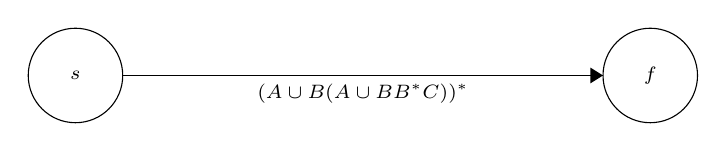
\begin{tikzpicture}[scale=0.2]
\tikzstyle{every node}+=[inner sep=0pt]
\draw [black] (15.7,-24) circle (3);
\draw (15.7,-24) node {$s$};
\draw [black] (52.2,-24) circle (3);
\draw (52.2,-24) node {$f$};
\draw [black] (18.7,-24) -- (49.2,-24);
\fill [black] (49.2,-24) -- (48.4,-23.5) -- (48.4,-24.5);
\draw (33.95,-24.5) node [below] {$(A \cup B(A \cup BB^* C))^*$};
\end{tikzpicture}
\end{center}

As can be seen from the result, the regular expression of the machine doesn't have to end with 'C'. However, we solve this problem by applying a simple trick. The thing is, if a word ends with 'C', then there must be $BB^* C$ part. The different ways that we can use this part in a word is $A^* (BA^*) (BB^* C)^*$. What we did is we concatenated the regular expression, and added kleene star to the elements that are connected with a union in order to find all the strings that ends with 'C'.


\section*{Answer for Q3}

In order to find the DFA representation of the whole system, there are some important points we must consider:\\
\\
$-$ Although the NFAs take the outputs (A,B,C) of the Mealy Machine; after we apply the DFA conversion to the whole system, the automata will still take the inputs in format (a,b). So, we must construct the DFA with the alphabet (a,b) not (A,B,C).\\
$-$ We can modify the NFAs $N_2$ and $N_3$ in order to make the DFA conversion more applicable. We  will analyze the regular expression of the Mealy Machine part by part to achieve our goal. An example for this modification is, in the NFA $N_3$ there is a part which accepts strings that has "CC":\\

\begin{center}
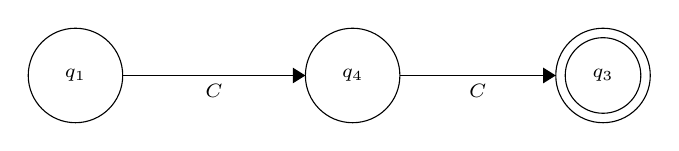
\begin{tikzpicture}[scale=0.2]
\tikzstyle{every node}+=[inner sep=0pt]
\draw [black] (19.3,-24.6) circle (3);
\draw (19.3,-24.6) node {$q_1$};
\draw [black] (36.9,-24.6) circle (3);
\draw (36.9,-24.6) node {$q_4$};
\draw [black] (52.8,-24.6) circle (3);
\draw (52.8,-24.6) node {$q_3$};
\draw [black] (52.8,-24.6) circle (2.4);
\draw [black] (22.3,-24.6) -- (33.9,-24.6);
\fill [black] (33.9,-24.6) -- (33.1,-24.1) -- (33.1,-25.1);
\draw (28.1,-25.1) node [below] {$C$};
\draw [black] (39.9,-24.6) -- (49.8,-24.6);
\fill [black] (49.8,-24.6) -- (49,-24.1) -- (49,-25.1);
\draw (44.85,-25.1) node [below] {$C$};
\end{tikzpicture}
\end{center}

   
However, we can't give a string like that to $N_3$ because Mealy Machines doesn't give outputs in that form. So we simply delete that part and so on..\\

After all of the modifications $N_2$ and $N_3$ will look like:\\

$-$$N_2$\\
\begin{center}
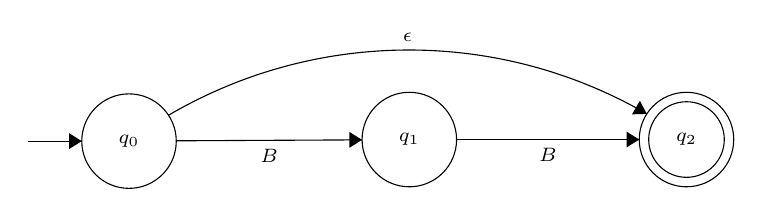
\begin{tikzpicture}[scale=0.2]
\tikzstyle{every node}+=[inner sep=0pt]
\draw [black] (15.6,-14.6) circle (3);
\draw (15.6,-14.6) node {$q_0$};
\draw [black] (33.4,-14.5) circle (3);
\draw (33.4,-14.5) node {$q_1$};
\draw [black] (51,-14.5) circle (3);
\draw (51,-14.5) node {$q_2$};
\draw [black] (51,-14.5) circle (2.4);
\draw [black] (9.2,-14.6) -- (12.6,-14.6);
\fill [black] (12.6,-14.6) -- (11.8,-14.1) -- (11.8,-15.1);
\draw [black] (18.6,-14.58) -- (30.4,-14.52);
\fill [black] (30.4,-14.52) -- (29.6,-14.02) -- (29.6,-15.02);
\draw (24.5,-15.06) node [below] {$B$};
\draw [black] (36.4,-14.5) -- (48,-14.5);
\fill [black] (48,-14.5) -- (47.2,-14) -- (47.2,-15);
\draw (42.2,-15) node [below] {$B$};
\draw [black] (18.109,-12.957) arc (120.37671:59.947:30.178);
\fill [black] (48.48,-12.87) -- (48.04,-12.04) -- (47.54,-12.9);
\draw (33.28,-8.31) node [above] {$\epsilon$};
\end{tikzpicture}
\end{center}

$-$$N_3$\\

\begin{center}
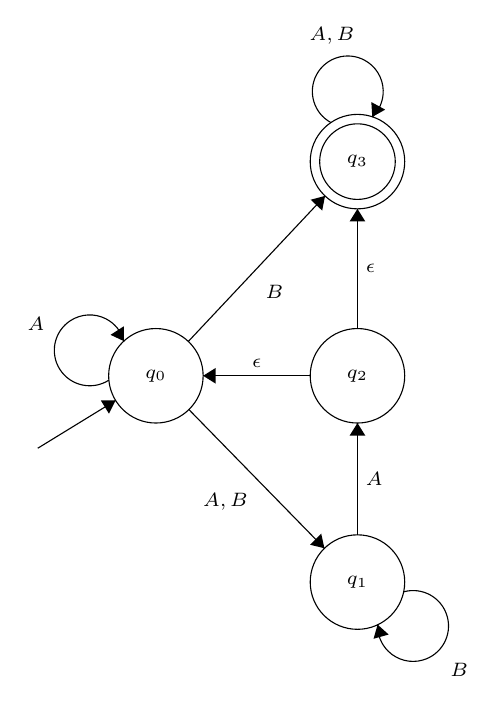
\begin{tikzpicture}[scale=0.2]
\tikzstyle{every node}+=[inner sep=0pt]
\draw [black] (17.1,-26.7) circle (3);
\draw (17.1,-26.7) node {$q_0$};
\draw [black] (29.9,-13.1) circle (3);
\draw (29.9,-13.1) node {$q_3$};
\draw [black] (29.9,-13.1) circle (2.4);
\draw [black] (29.9,-26.7) circle (3);
\draw (29.9,-26.7) node {$q_2$};
\draw [black] (29.9,-39.8) circle (3);
\draw (29.9,-39.8) node {$q_1$};
\draw [black] (19.16,-24.52) -- (27.84,-15.28);
\fill [black] (27.84,-15.28) -- (26.93,-15.52) -- (27.66,-16.21);
\draw (24.03,-21.37) node [right] {$B$};
\draw [black] (14.124,-26.972) arc (302.96249:14.96249:2.25);
\draw (10.05,-23.43) node [left] {$A$};
\fill [black] (15.07,-24.5) -- (15.06,-23.56) -- (14.22,-24.1);
\draw [black] (28.224,-10.626) arc (241.85331:-46.14669:2.25);
\draw (28.28,-5.71) node [above] {$A,B$};
\fill [black] (30.84,-10.26) -- (31.66,-9.8) -- (30.78,-9.32);
\draw [black] (29.9,-23.7) -- (29.9,-16.1);
\fill [black] (29.9,-16.1) -- (29.4,-16.9) -- (30.4,-16.9);
\draw (30.4,-19.9) node [right] {$\epsilon$};
\draw [black] (26.9,-26.7) -- (20.1,-26.7);
\fill [black] (20.1,-26.7) -- (20.9,-27.2) -- (20.9,-26.2);
\draw (23.5,-26.2) node [above] {$\epsilon$};
\draw [black] (29.9,-36.8) -- (29.9,-29.7);
\fill [black] (29.9,-29.7) -- (29.4,-30.5) -- (30.4,-30.5);
\draw (30.4,-33.25) node [right] {$A$};
\draw [black] (32.823,-40.422) arc (105.70984:-182.29016:2.25);
\draw (35.76,-45.4) node [right] {$B$};
\fill [black] (31.18,-42.5) -- (30.92,-43.4) -- (31.88,-43.13);
\draw [black] (19.2,-28.85) -- (27.8,-37.65);
\fill [black] (27.8,-37.65) -- (27.6,-36.73) -- (26.89,-37.43);
\draw (22.97,-34.72) node [left] {$A,B$};
\draw [black] (9.6,-31.3) -- (14.54,-28.27);
\fill [black] (14.54,-28.27) -- (13.6,-28.26) -- (14.12,-29.11);
\end{tikzpicture}
\end{center}



$-$So that we have the modified versions of the NFAs, now we will change the transition types from outputs of the Mealy Machine to inputs that Mealy Machine takes (a/A,b/B,a/C), and combine both $N_2$ and $N_3$ with the non-deterministic gate.\\
\\
Now, our system will look like this:


\begin{center}
\begin{tikzpicture}[scale=0.2]
\tikzstyle{every node}+=[inner sep=0pt]
\draw [black] (53.6,-39.3) circle (3);
\draw (53.6,-39.3) node {$q_3$};
\draw [black] (67.2,-26) circle (3);
\draw (67.2,-26) node {$q_6$};
\draw [black] (67.2,-26) circle (2.4);
\draw [black] (67.2,-39.3) circle (3);
\draw (67.2,-39.3) node {$q_5$};
\draw [black] (67.2,-51.4) circle (3);
\draw (67.2,-51.4) node {$q_4$};
\draw [black] (25.8,-51.4) circle (3);
\draw (25.8,-51.4) node {$gate$};
\draw [black] (26,-36.7) circle (3);
\draw (26,-36.7) node {$q_0$};
\draw [black] (26,-22.8) circle (3);
\draw (26,-22.8) node {$q_1$};
\draw [black] (26,-8.5) circle (3);
\draw (26,-8.5) node {$q_2$};
\draw [black] (26,-8.5) circle (2.4);
\draw [black] (55.74,-37.2) -- (65.06,-28.1);
\fill [black] (65.06,-28.1) -- (64.13,-28.3) -- (64.83,-29.01);
\draw (61.42,-33.13) node [below] {$b$};
\draw [black] (50.624,-39.572) arc (302.96249:14.96249:2.25);
\draw (46.55,-36.03) node [left] {$a$};
\fill [black] (51.57,-37.1) -- (51.56,-36.16) -- (50.72,-36.7);
\draw [black] (65.559,-23.503) arc (241.04957:-46.95043:2.25);
\draw (65.91,-18.65) node [above] {$a,b$};
\fill [black] (68.18,-23.18) -- (69.01,-22.72) -- (68.13,-22.24);
\draw [black] (67.2,-36.3) -- (67.2,-29);
\fill [black] (67.2,-29) -- (66.7,-29.8) -- (67.7,-29.8);
\draw (67.7,-32.65) node [right] {$\epsilon$};
\draw [black] (64.2,-39.3) -- (56.6,-39.3);
\fill [black] (56.6,-39.3) -- (57.4,-39.8) -- (57.4,-38.8);
\draw (60.4,-38.8) node [above] {$\epsilon$};
\draw [black] (67.2,-48.4) -- (67.2,-42.3);
\fill [black] (67.2,-42.3) -- (66.7,-43.1) -- (67.7,-43.1);
\draw (67.7,-45.35) node [right] {$a$};
\draw [black] (70.123,-52.022) arc (105.70984:-182.29016:2.25);
\draw (73.06,-57) node [right] {$b$};
\fill [black] (68.48,-54.1) -- (68.22,-55) -- (69.18,-54.73);
\draw [black] (55.84,-41.29) -- (64.96,-49.41);
\fill [black] (64.96,-49.41) -- (64.69,-48.5) -- (64.03,-49.25);
\draw (58.69,-45.84) node [below] {$a,b$};
\draw [black] (28.55,-50.2) -- (50.85,-40.5);
\fill [black] (50.85,-40.5) -- (49.92,-40.36) -- (50.32,-41.27);
\draw (40.6,-45.86) node [below] {$\epsilon$};
\draw [black] (25.84,-48.4) -- (25.96,-39.7);
\fill [black] (25.96,-39.7) -- (25.45,-40.49) -- (26.45,-40.51);
\draw (26.42,-44.05) node [right] {$\epsilon$};
\draw [black] (26,-33.7) -- (26,-25.8);
\fill [black] (26,-25.8) -- (25.5,-26.6) -- (26.5,-26.6);
\draw (26.5,-29.75) node [right] {$b$};
\draw [black] (26,-19.8) -- (26,-11.5);
\fill [black] (26,-11.5) -- (25.5,-12.3) -- (26.5,-12.3);
\draw (26.5,-15.65) node [right] {$b$};
\draw [black] (28.079,-6.353) arc (163.65382:-124.34618:2.25);
\draw (33.12,-5.46) node [right] {$a$};
\fill [black] (28.97,-8.84) -- (29.6,-9.55) -- (29.88,-8.59);
\draw [black] (23.918,-34.544) arc (-140.56793:-219.43207:18.805);
\fill [black] (23.92,-10.66) -- (23.02,-10.96) -- (23.8,-11.59);
\draw (19.14,-22.6) node [left] {$\epsilon$};
\end{tikzpicture}
\end{center}


$-$ Now, we will apply the NFA to DFA algorithm to the system above. The final DFA will look like:

\begin{center}
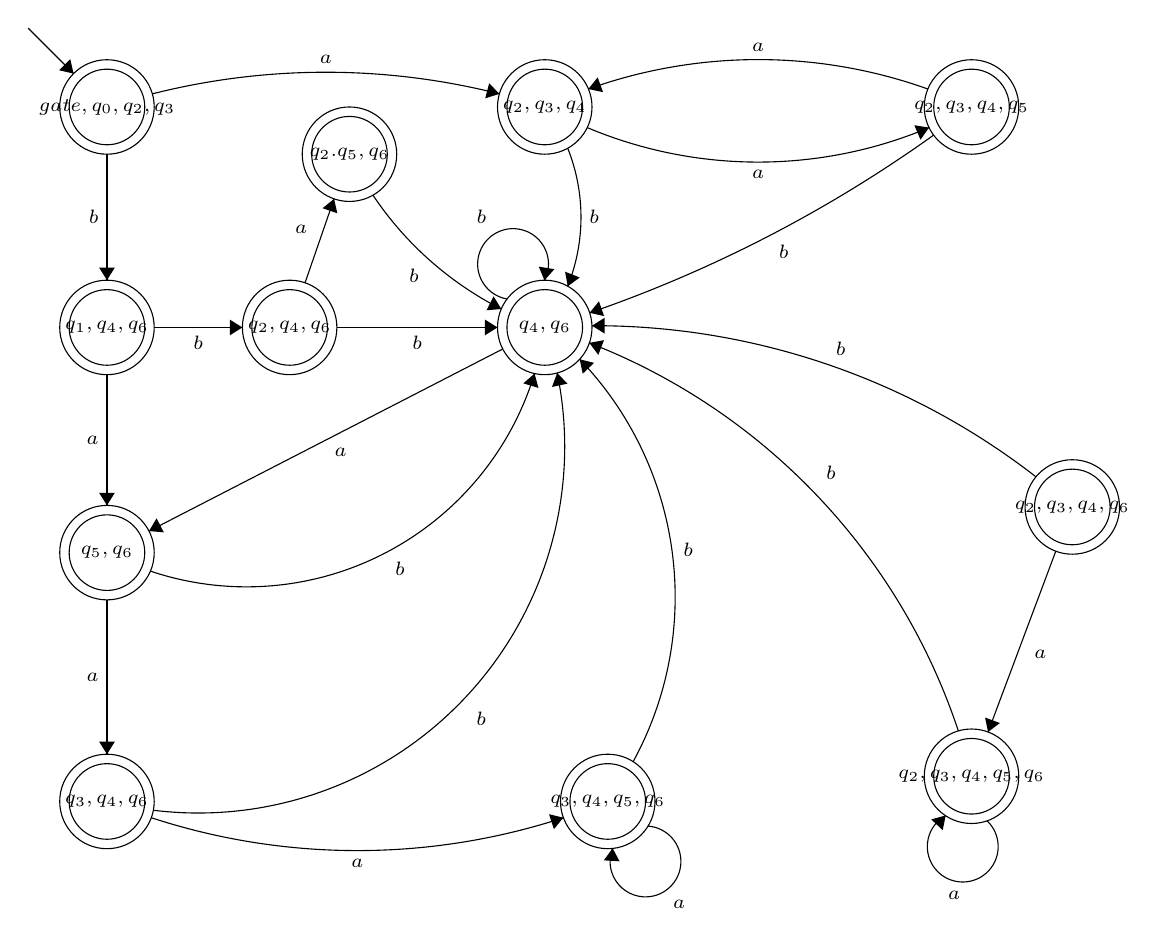
\begin{tikzpicture}[scale=0.2]
\tikzstyle{every node}+=[inner sep=0pt]
\draw [black] (8,-7.1) circle (3);
\draw (8,-7.1) node {$gate,q_0,q_2,q_3$};
\draw [black] (8,-7.1) circle (2.4);
\draw [black] (8,-21.1) circle (3);
\draw (8,-21.1) node {$q_1,q_4,q_6$};
\draw [black] (8,-21.1) circle (2.4);
\draw [black] (8,-35.4) circle (3);
\draw (8,-35.4) node {$q_5,q_6$};
\draw [black] (8,-35.4) circle (2.4);
\draw [black] (8,-51.2) circle (3);
\draw (8,-51.2) node {$q_3,q_4,q_6$};
\draw [black] (8,-51.2) circle (2.4);
\draw [black] (39.8,-51.2) circle (3);
\draw (39.8,-51.2) node {$q_3,q_4,q_5,q_6$};
\draw [black] (39.8,-51.2) circle (2.4);
\draw [black] (35.8,-7.1) circle (3);
\draw (35.8,-7.1) node {$q_2,q_3,q_4$};
\draw [black] (35.8,-7.1) circle (2.4);
\draw [black] (62.9,-7.1) circle (3);
\draw (62.9,-7.1) node {$q_2,q_3,q_4,q_5$};
\draw [black] (62.9,-7.1) circle (2.4);
\draw [black] (35.8,-21.1) circle (3);
\draw (35.8,-21.1) node {$q_4,q_6$};
\draw [black] (35.8,-21.1) circle (2.4);
\draw [black] (19.6,-21.1) circle (3);
\draw (19.6,-21.1) node {$q_2,q_4,q_6$};
\draw [black] (19.6,-21.1) circle (2.4);
\draw [black] (23.4,-10.1) circle (3);
\draw (23.4,-10.1) node {$q_2.q_5,q_6$};
\draw [black] (23.4,-10.1) circle (2.4);
\draw [black] (69.3,-32.5) circle (3);
\draw (69.3,-32.5) node {$q_2,q_3,q_4,q_6$};
\draw [black] (69.3,-32.5) circle (2.4);
\draw [black] (62.9,-49.6) circle (3);
\draw (62.9,-49.6) node {$q_2,q_3,q_4,q_5,q_6$};
\draw [black] (62.9,-49.6) circle (2.4);
\draw [black] (10.881,-6.267) arc (104.21441:75.78559:44.873);
\fill [black] (32.92,-6.27) -- (32.27,-5.59) -- (32.02,-6.55);
\draw (21.9,-4.39) node [above] {$a$};
\draw [black] (60.202,-8.41) arc (-67.17729:-112.82271:27.979);
\fill [black] (60.2,-8.41) -- (59.27,-8.26) -- (59.66,-9.18);
\draw (49.35,-11.1) node [below] {$a$};
\draw [black] (38.573,-5.959) arc (109.67524:70.32476:32.008);
\fill [black] (38.57,-5.96) -- (39.5,-6.16) -- (39.16,-5.22);
\draw (49.35,-3.59) node [above] {$a$};
\draw [black] (8,-10.1) -- (8,-18.1);
\fill [black] (8,-18.1) -- (8.5,-17.3) -- (7.5,-17.3);
\draw (7.5,-14.1) node [left] {$b$};
\draw [black] (8,-24.1) -- (8,-32.4);
\fill [black] (8,-32.4) -- (8.5,-31.6) -- (7.5,-31.6);
\draw (7.5,-28.25) node [left] {$a$};
\draw [black] (8,-38.4) -- (8,-48.2);
\fill [black] (8,-48.2) -- (8.5,-47.4) -- (7.5,-47.4);
\draw (7.5,-43.3) node [left] {$a$};
\draw [black] (36.985,-52.234) arc (-71.87654:-108.12346:42.064);
\fill [black] (36.98,-52.23) -- (36.07,-52.01) -- (36.38,-52.96);
\draw (23.9,-54.82) node [below] {$a$};
\draw [black] (42.346,-52.765) arc (86.1574:-201.8426:2.25);
\draw (44.34,-57.41) node [below] {$a$};
\fill [black] (40.11,-54.17) -- (39.55,-54.94) -- (40.55,-55);
\draw [black] (11,-21.1) -- (16.6,-21.1);
\fill [black] (16.6,-21.1) -- (15.8,-20.6) -- (15.8,-21.6);
\draw (13.8,-21.6) node [below] {$b$};
\draw [black] (68.25,-35.31) -- (63.95,-46.79);
\fill [black] (63.95,-46.79) -- (64.7,-46.22) -- (63.76,-45.87);
\draw (66.86,-41.87) node [right] {$a$};
\draw [black] (63.88,-52.423) arc (46.87498:-241.12502:2.25);
\draw (61.8,-56.88) node [below] {$a$};
\fill [black] (61.26,-52.09) -- (60.34,-52.34) -- (61.07,-53.02);
\draw [black] (33.419,-19.295) arc (260.56505:-27.43495:2.25);
\draw (31.79,-14.56) node [above] {$b$};
\fill [black] (35.78,-18.11) -- (36.41,-17.4) -- (35.42,-17.24);
\draw [black] (33.13,-22.47) -- (10.67,-34.03);
\fill [black] (10.67,-34.03) -- (11.61,-34.11) -- (11.15,-33.22);
\draw (22.84,-28.75) node [below] {$a$};
\draw [black] (22.6,-21.1) -- (32.8,-21.1);
\fill [black] (32.8,-21.1) -- (32,-20.6) -- (32,-21.6);
\draw (27.7,-21.6) node [below] {$b$};
\draw [black] (36.591,-23.992) arc (11.60176:-97.05215:23.265);
\fill [black] (36.59,-23.99) -- (36.26,-24.88) -- (37.24,-24.67);
\draw (31.43,-45.92) node [right] {$b$};
\draw [black] (38.017,-23.117) arc (43.76843:-28.62902:21.827);
\fill [black] (38.02,-23.12) -- (38.21,-24.04) -- (38.93,-23.35);
\draw (44.57,-35.19) node [right] {$b$};
\draw [black] (33.04,-19.931) arc (-116.94121:-146.21105:21.56);
\fill [black] (33.04,-19.93) -- (32.55,-19.12) -- (32.1,-20.01);
\draw (27.49,-17.33) node [below] {$b$};
\draw [black] (38.634,-22.082) arc (68.73317:18.38204:39.961);
\fill [black] (38.63,-22.08) -- (39.2,-22.84) -- (39.56,-21.91);
\draw (53.63,-30.32) node [right] {$b$};
\draw [black] (38.797,-20.99) arc (90.22662:52.18666:45.693);
\fill [black] (38.8,-20.99) -- (39.6,-21.49) -- (39.6,-20.49);
\draw (54.6,-22.89) node [above] {$b$};
\draw [black] (60.491,-8.888) arc (-54.42285:-70.93493:85.591);
\fill [black] (38.65,-20.17) -- (39.57,-20.38) -- (39.24,-19.44);
\draw (50.97,-15.82) node [below] {$b$};
\draw [black] (20.58,-18.26) -- (22.42,-12.94);
\fill [black] (22.42,-12.94) -- (21.69,-13.53) -- (22.63,-13.85);
\draw (20.74,-14.86) node [left] {$a$};
\draw [black] (37.255,-9.714) arc (21.81762:-21.81762:11.801);
\fill [black] (37.26,-18.49) -- (38.02,-17.93) -- (37.09,-17.56);
\draw (38.6,-14.1) node [right] {$b$};
\draw [black] (35.153,-24.026) arc (-16.96739:-108.59108:19.13);
\fill [black] (35.15,-24.03) -- (34.44,-24.65) -- (35.4,-24.94);
\draw (26.6,-35.96) node [below] {$b$};
\draw [black] (3,-2.1) -- (5.88,-4.98);
\fill [black] (5.88,-4.98) -- (5.67,-4.06) -- (4.96,-4.77);
\end{tikzpicture}
\end{center}


$-$By applying these steps, we converted the system to a DFA without worrying about Mealy Machine.

\end{document}
